\documentclass{sig-alternate}
\usepackage{algorithm,algpseudocode}

\begin{document}

\conferenceinfo{HPDC}{'12 Delft, The Netherlands}
% \CopyrightYear{2007} % Allows default copyright year (20XX) to be over-ridden
% - IF NEED BE. \crdata{0-12345-67-8/90/01}  % Allows default copyright data
% (0-89791-88-6/97/05) to be over-ridden - IF NEED BE.

\title{Cost- and Deadline-constrained Scheduling of Scientific Workflow Ensembles in IaaS Clouds}
% \subtitle{[Extended Abstract]}

\numberofauthors{2}
\author{
    \alignauthor Maciej Malawski and Jarek Nabrzyski\\
       \affaddr{University of Notre Dame}\\
       \affaddr{Center for Research Computing}\\
       \affaddr{111 Information Technology Center}\\
       \affaddr{Notre Dame, IN, USA}\\
       \email{\{mmalawsk,naber\}@nd.edu}
    \alignauthor Gideon Juve and Ewa Deelman\\
       \affaddr{USC Information Sciences Institute}\\
       \affaddr{4676 Admiralty Way}\\
       \affaddr{Marina del Rey, CA, USA}\\
       \email{\{gideon,deelman\}@isi.edu}
}

\maketitle
 
\begin{abstract}
Abstract goes here.
\end{abstract}

%\category{H.4}{Information Systems Applications}{Miscellaneous}
%\category{D.2.8}{Software Engineering}{Metrics}[complexity measures, performance measures]

%\terms{Theory}

\keywords{Scientific workflows, DAG scheduling, simulation}

\section{Introduction}

Scientific workflows, usually represented as directed acyclic graphs (DAG), are
the important class of applications that have been studied in the context of
resource management and scheduling on grid and utility computing systems.
However, large computational applications are not just individual workflows but
rather sets of inter-related workflows grouped in {\em ensembles}. All the
workflows in an ensemble typically have a similar structure, but they differ by
input data, number of tasks and individual tasks sizes. A good example of
scientific workflow ensemble comes from the CyberShake
application~\cite{Callaghan11}, which calculates seismic hazards for a given
geographical region such as California. In order to produce a hazard map, the
hazard curves need to be computed for a set of geographical sites, while each
site requires running a single complex scientific workflow. Workflows for each
site may differ not only by their parameters, but also by priority; e.g. some of
the points on the map correspond to urban areas or strategic locations such as
power plants, whereas others may be located in low populated regions. Another
examples of workflow ensembles come from astronomical applications, such as
Montage~\cite{Deelman08} or search for Earth-like planets from Kepler project
data~\cite{vockler11}, where multiple workflows are typically required to
process data covering different parts of the sky.
 
Infrastructure-as-a-service (Iaas) clouds offer capabilities of creating
(provisioning) computational resources on demand in a pay-per-use model and are regarded by
scientific community as a potentially attractive source of computing
resources~\cite{Ostermann10,Keahey09}. In contrast to clusters and grids which
typically offer best-effort resource provisioning capabilities, clouds give more
flexibility in terms of creating a controlled and managed computing environment
with the ability of adjusting resource capacity to the computing demands, often
called auto-scaling. Giving the users more control, however, clouds also require
developing new methods of task scheduling and resource provisioning. The
resource management decisions in cloud scenarios not only have to take into
account performance related metrics such as workflow makespan or resource
utilization, but also budget considerations, since the resources from public
(commercial) cloud providers are usually not free~\cite{Durkee10}.

In this paper, to get insight into these resource management challenges for
scietific workflow on clouds, we address a new important problem of maximizing
the number of completed workflows from an ensemble under both budget and
deadline constraints. The motivation is to answer the fundamental question of a
researcher: how much work can be completed in a limited budget and timeframe of
a research project. The goals of this paper are to discuss and assess possible
static and dynamic strategies for both task scheduling and resource
provisioning. Based on the knowledge of workflow scheduling algorithms we
analyze strategies for on-line scheduling of individual tasks as well as static
algorithms that rely on the information about the workflow structure (critical
paths and workflow levels) and estimates of task runtimes. In addition, we
analyze a hybrid workflow-aware dynamic scheduling algorithm, which uses the
workflow structure information to estimate which workflows should be rejected
from the ensemble due to the constraints. As methodology in the study of the
proposed algorithms we use simulation techniques. We have developed cloud workflow simulator based on
CloudSim~\cite{Calheiros11}, which models the infrastructure and the application. The
algorithms are subject to evaluation on a set of scientific workflow ensembles with a broad range of
budget and deadline parameters. 

The paper is organized as follows [\ldots]

\section{Related Work}
General policy and rule-based approaches to dynamic provisioning (e.g. Amazon Auto Scaling\footnote{http://aws.amazon.com/autoscaling} and RightScale\footnote{http://www.rightscale.com}).

Policy-based approaches for scientific workloads (e.g. \cite{Marshall2010, Kim2011}). Our approach is different in that we consider workflows, while policy based approaches typically consider bags of independent tasks or unpredictable batch workloads. This enables us to take advantage of scheduling heuristics that cannot be applied to independent tasks.

Deadline-constrained cost-minimization workflow scheduling. Our work is different from \cite{Yu2005, Abrishami2010} in that we consider ensembles of workflows in IaaS clouds, which allow one to provision resources on a per-hour billing model, rather than utility grids, which allow one to choose from a pool of existing resources with a per-job billing model. Our work is different from \cite{Mao2011} in that we consider ensembles of workflows rather than unpredictable workloads containing workflows. We also have budget constraints rather than cost minimization as a goal. In other words, we assume that there is more work to be done than the available budget, so some work must be rejected. Therefore cost is not something we optimize, but rather a constraint.

Budget-constrained workflow scheduling \cite{Sakellariou2007}.

Bi-criteria scheduling and multi-criteria scheduling. These approaches are similar to ours in that we have two scheduling criteria: cost and makespan. The challenge in multi-criteria scheduling is to derive an objective function that takes into account all of the criteria. These approaches typically use metaheuristics that run for a long time before producing good results.

\section{Problem Description}
\subsection{Resource Model}
Describe the Amazon EC2 resource model. Instances are requested on-demand. Instance pricing is per-hour. Multiple VM types are available, but for this paper we focus on a single VM type because we assume that there will typically be one VM type with the best price/performance ratio for the application.

\subsection{Application Model}
The target applications for this paper are scientific workflows that can be modeled as Directed Acyclic Graphs (DAGs).

We assume that we have runtime estimates for each task in the workflow.

Currently we do not consider data sizes, but rather assume that data is stored in a shared cloud storage system such as Amazon S3 and that data transfer times are included in task runtime estimates. Further, data transfer times are equal across the VMs.

An ensemble consists of several related workflows. Each workflow is given a priority.

The goal is to complete as many workflows as possible given a budget and a deadline.

\section{Algorithms}

\subsection{Static Provisioning Dynamic Scheduling (SPDS)}
\label{sec:spds}
This is the simplest strategy based on static provisioning of resources and
on-line scheduling of workflow tasks. Given the budget $B$ and deadline $d$
together with the hourly price $p$ of a VM it is possible to compute the number
of VMs $N_{VM}$ to provision so that they consume the whole budget before the
deadline. 

\begin{equation}
\label{eq:static-plan}
N_{VM} = \lceil B / d / p \rceil
\end{equation}

Although simple, such provisioning plan has the advantage that it
minimizes the number of provisioning and deprovisioning requests.
Once the resources are provisioned, the tasks are scheduled to VMs using dynamic
priority-based Algorithm~\ref{alg:ds}. 

\begin{algorithm}
\caption{Priority-based scheduling}
\label{alg:ds}
\begin{algorithmic}[1]
\Procedure{schedule}{}
    \State $Q\gets set\ of\ released\ tasks$
    \State $P\gets empty\ priority\ queue$
    \While{$Q \neq \emptyset$}
    	\For{$task\ t\in Q$}
    		\State \Call{Insert}{$t,P$} 
    	\EndFor
    	\While{$FreeVMs \neq \emptyset \wedge P \neq \emptyset $}
    		\State $VM\gets$ \Call{SelectRandom}{$FreeVMs$}
    		\State $t\gets$ \Call{Pop}{$P$}
    		\State \Call{Submit}{$t,VM$}
    	\EndWhile
    	\State \Call{Wait}{$task\ finished$}
    	\State \Call{Update}{$Q$}
    \EndWhile
\EndProcedure
\end{algorithmic} 
\end{algorithm}

Initially all the
released tasks from all the workflows are submitted to the queue $Q$. Then, they
are inserted into priority queue $P$ based on the priority of workflows. If
there are free VMs available, the tasks from the priority queue are submitted to
the randomly choosen VMs. The process is repeated each time a task finishes.
Using the priority queue guarantees that tasks from lower priority workflows are
always submitted later than the higher priority ones and that the lower priority
tasks can occupy idle VMs. However, as there is no preemption, long-running
low-priority tasks may delay execution of high-priority tasks when such ones
become ready. Fig.~\ref{fig:spss-example} shows the example plan generated using
SPSS algorithm. It can be seen that tasks from lower priority workflows can fill
idle time of provisioned virtual machines.

\begin{figure}[htb] 
\centering
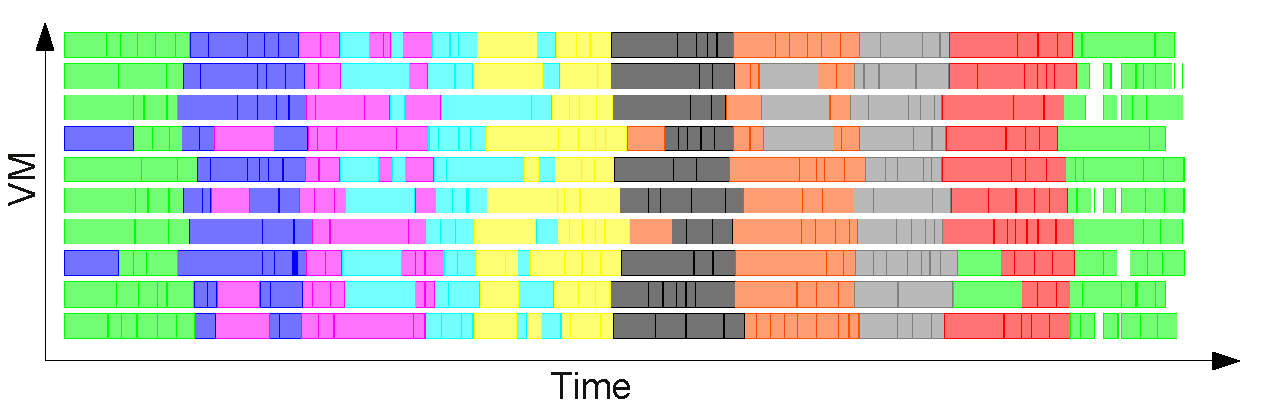
\includegraphics[width=1.0\columnwidth]{figures/spds-gantt}
 \caption{Example of schedule generated using SPSS algorithm: tasks are labelled
 by colors depending on the workflow. }
\label{fig:spss-example}
\end{figure}

\subsection{Dynamic Provisioning Dynamic Scheduling (DPDS)}

Static provisioning plan used in SPDS algorithm allows no changes to resource
pool at runtime. However, such plan may not be optimal when resource demand
changes during execution of workflows. In policy-based provisioning
(or auto-scaling) systems the metrics such as resource
utilization or queue length are typicaly used to estimate curret resource
demand. Our DPDS algorithm is based on resource utilization: the provisioner
module periodically computes utilization as the percentage of idle VMs. The
provisioner algorithm detects which VMs are finishing their hourly billing cycle
during the next provisioning period and decides whether they should continue
running, should be terminated or new VMs should be provisioned: see
Algorithm~\ref{alg:prov}.

\begin{algorithm}
\caption{Dynamic provisioner}
\label{alg:prov}
\begin{algorithmic}[1]
\Require $c$: consumed budget; $b$: total budget; $d$: deadline; $p$: price;
$t$: current time; $u_h$: upper utilization thershold; $u_l$: lower utilization
threshold.
\Procedure{provision}{}
    \State $V_C\gets set\ of\ VMs\ completing\ billing\ cycle$
    \State $n_T\gets\ 0$ \Comment{number of VMs to terminate} 
    \If{$ b - c < p * |V_C| \vee t > d $ }
    	\State $V_R\gets set\ of\ running\ VMs$
    	\State $n_T\gets |V_R| - \lfloor(b-c)/p\rfloor$ 
    	\State $V_T\gets select\ n_T VMs\ to\ terminate\ from\ V_C$
    	\State \Call{Terminate}{$V_T$}
    \Else 
    	\If{$u>u_h$}
    		\State \Call{Start}{$new\ VM$}
    	\EndIf
    	\If{$u<u_l$}
    		\State $V_F\gets free\ (idle)\ VMs$
    		\State $n_T\gets \lceil|V_F|/2\rceil$ 
    		\State \Call{Terminate}{$V_T$}
    	\EndIf 
    \EndIf
\EndProcedure
\end{algorithmic} 
\end{algorithm}

The number of instances to terminate $n_T$ computed in line 6 is the number that
would overrun the budget if not terminated. On the other hand $n_T$ computed in
line 15 prevents terminating all the instances too quickly, but makes sure that
if there is only one instance left it should be terminated. However, the
termination process is not immediate: to make sure that VMs that have been
already paid for are not terminated prematurely the {\em Terminate()} procedure
terminates only these instances that are close to the end of their billing
cycle. The remaining time threshold is calculated as a sum of provisioner
interval and estimated termination delay. This guarantees that no VMs can
overrun the assigned budget. To avoid uncontrolled increase of number of
instances, which may happen in the case of highly parallel workflows,
provisioner checks also the maximum scaling factor from the initial number of
provisioned VMs and prohibits starting new ones when this threshold is reached.


\subsection{Workflow-Aware DPDS (WA-DPDS)}

\subsection{Static Provisioning Static Scheduling (SPSS)}

We assume that the workflows are very wide such that the critical path of any given workflow is much less than the deadline.

The approach is to schedule each workflow in the ensemble in priority order, rejecting any workflows that cannot be completed by the deadline or that cause the cost of the plan to exceed the budget. Once the plan is complete, then the workflows are executed according to the plan.

\begin{algorithm}
\caption{Ensemble planning algorithm}
\label{alg:admit}
\begin{algorithmic}[1]
\Require $W$: workflow ensemble; $b$: budget; $d$: deadline
\Ensure Schedule as much of $W$ as possible given $b$ and $d$
\Procedure{PlanEnsemble}{$W,b,d$}
    \State $P\gets empty\ plan$
    \State $A\gets \emptyset$ \Comment{Set of admitted DAGs}
    \For{$w\ in\ W$}
        \State $P^\prime \gets$\ \Call{PlanDAG}{$w,P,d$}
        \If{$P^\prime\ is\ a\ valid\ plan$}
            \If{$Cost(P^\prime) \le b$}
                \State $P\gets\ P^\prime$ \Comment{Accept new plan}
                \State $A \gets A\ +\ w$ \Comment{Admit w}
            \EndIf
        \EndIf
    \EndFor
    \State \textbf{return} $P,A$
\EndProcedure
\end{algorithmic} 
\end{algorithm}


\begin{algorithm}
\caption{DAG planning algorithm}
\label{alg:plandag}
\begin{algorithmic}[1]
\Require $w$: DAG; $P$: current plan; $d$: deadline
\Ensure Create plan for $w$ that minimizes cost and meets deadline $d$
\Procedure{PlanDAG}{$w,P,d$}
    \State $P^\prime\gets$ copy of $P$
    \State \Call{DeadlineDistribution}{w,d}
    \For{$t\ in\ w\ sorted\ by\ Deadline(t)$}
        \State Choose resource r in $P^\prime$ that minimizes Cost(t)
        \If{$AFT(t,r) < Deadline(t)$}
            \State Schedule(t,r)
        \Else
            \State Provision a new resource r
            \State Schedule(t,r)
        \EndIf
    \EndFor
    \State \textbf{return} $P^\prime$
\EndProcedure
\end{algorithmic} 
\end{algorithm}


\begin{algorithm}
\caption{Deadline distribution algorithm}
\label{alg:deadlinedistribution}
\begin{algorithmic}[1]
\Require $w$: DAG; $d$: global deadline
\Ensure Assign sub-deadlines to each task in w
\Procedure{DeadlineDistribution}{$w,d$}
    \State $T \gets$ total number of tasks in $w$
    \State $R \gets$ total runtime of tasks in $w$
    \State $CP \gets$ length of critical path of $w$
    \State assign $Level(t)$ to each task $t$ in $w$
    \For{level $l\ \in w$}
        \State $Tasks(l) \gets$ number of tasks in $l$
        \State $Runtime(l) \gets$ runtime of tasks in $l$
        \State $r \gets \alpha * (Runtime(l)/R)$
        \State $t \gets (1-\alpha) * (Tasks(l)/T)$
        \State $FT(l) \gets (r + t) * (d - CP)$
    \EndFor
    \For{task $t \in w$}
        \State $LST(t) \gets \max(Deadline(p))\ for\ p \in Pred(t)$
        \State $Deadline(t) \gets LST(t) + RT(t) + FT(Level(t))$
    \EndFor
\EndProcedure
\end{algorithmic} 
\end{algorithm}

\begin{equation}
\label{eq:scaling}
FT(l) = \left[{\alpha}*\frac{T_l}{t}\right] + \left[{(1 - \alpha)}*\frac{R_l}{r} \right]
\end{equation}

\section{Performance Evaluation}

\subsection{Simulator}

\subsection{Scenarios}

\subsection{Results}


\begin{figure*}[htb] 
\centering
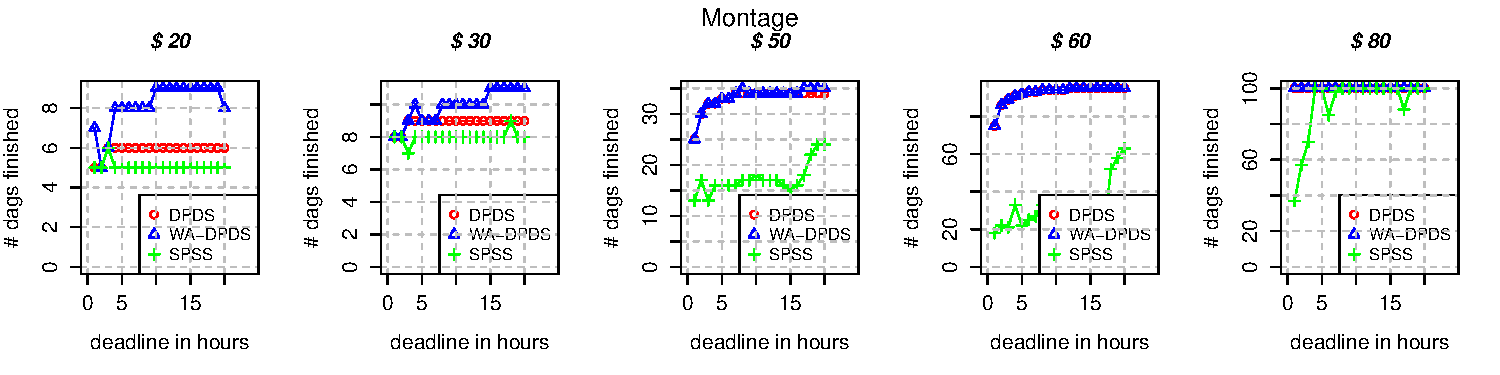
\includegraphics[width=1.0\textwidth]{figures/MONTAGE-n-1000-8-dagh1-20m0.pdf}
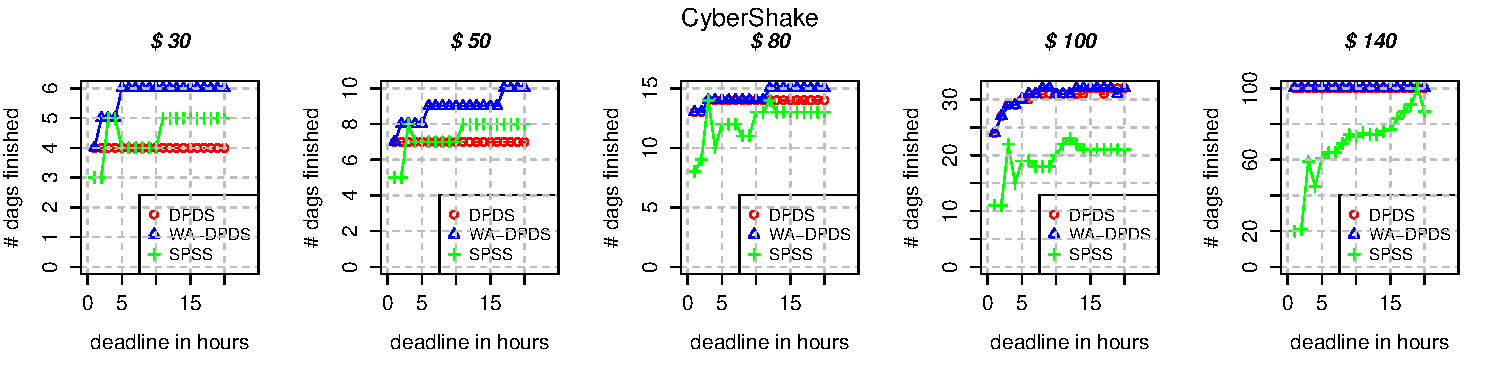
\includegraphics[width=1.0\textwidth]{figures/CYBERSHAKE-n-1000-8-dagh1-20m0.pdf}
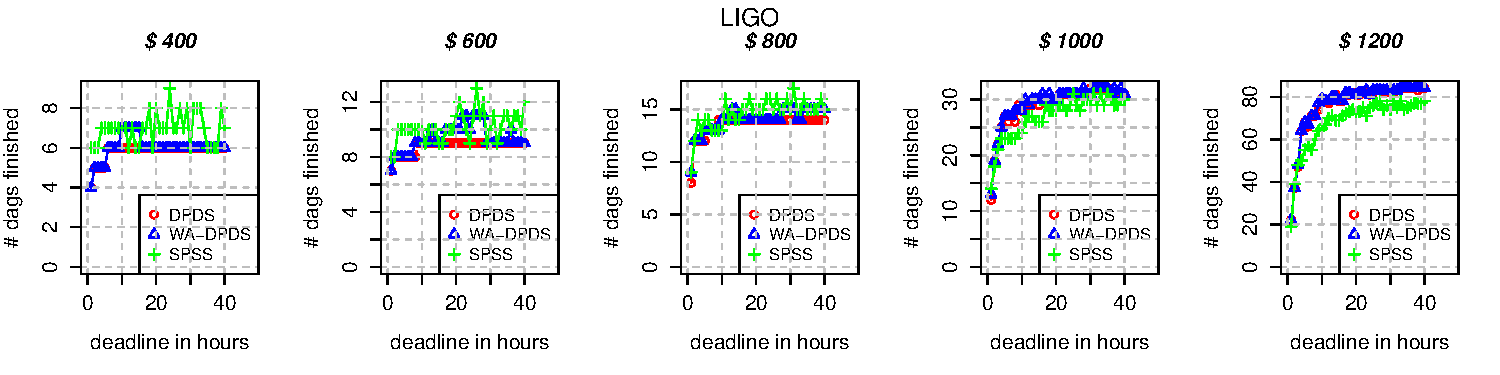
\includegraphics[width=1.0\textwidth]{figures/LIGO-n-1000-8-dagh1-40m0.pdf}
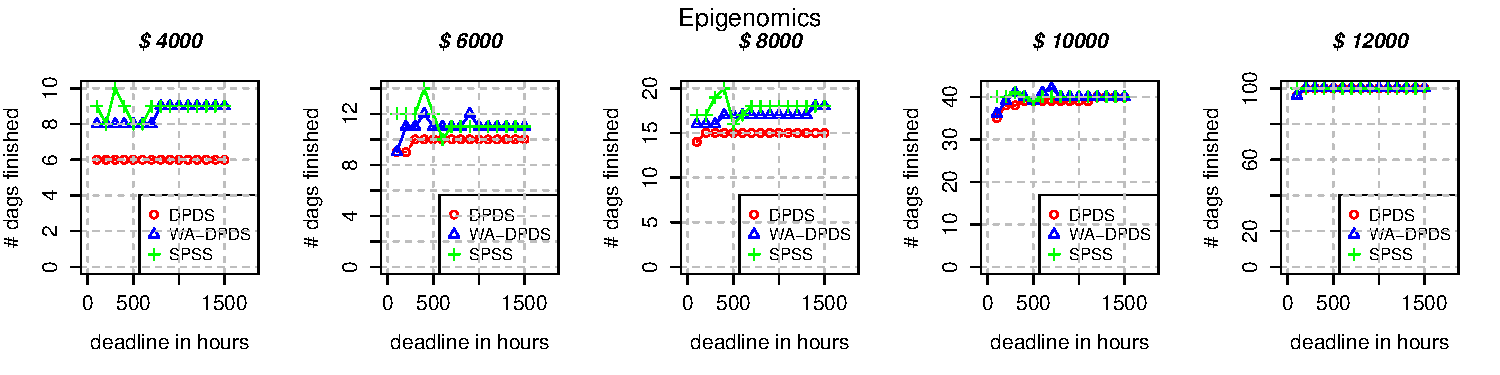
\includegraphics[width=1.0\textwidth]{figures/GENOME-n-1000-8-dagh100-1500m0.pdf}
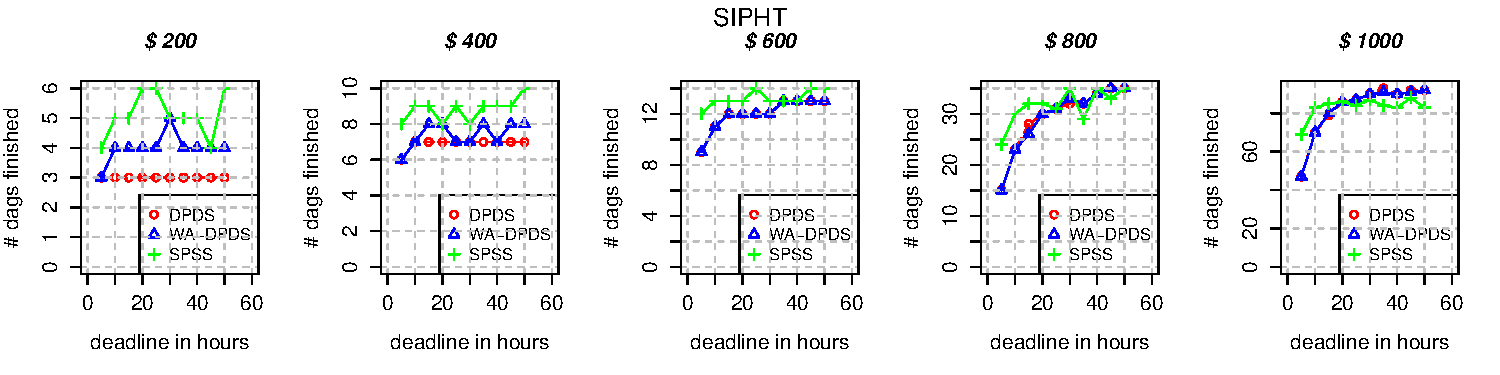
\includegraphics[width=1.0\textwidth]{figures/SIPHT-n-1000-8-dagh5-50m0.pdf}
\caption{Comparison of DPDS, AW-DPDS and SPSS algorithms for ensembles of 100
Pareto-distributed workflows}
\label{fig:}
\end{figure*}


\begin{figure*}[htb] 
\centering
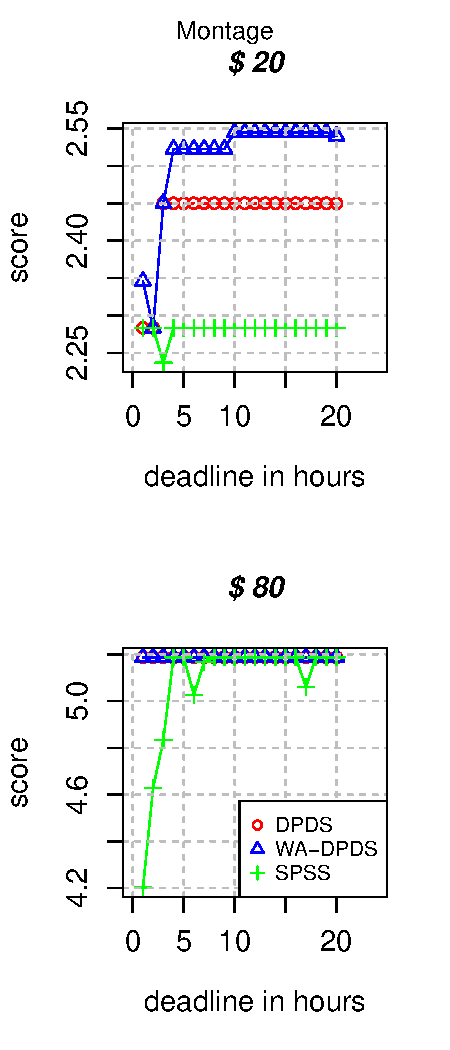
\includegraphics[width=1.0\textwidth]{figures/score-MONTAGE-n-1000-8-dagh1-20m0.pdf}
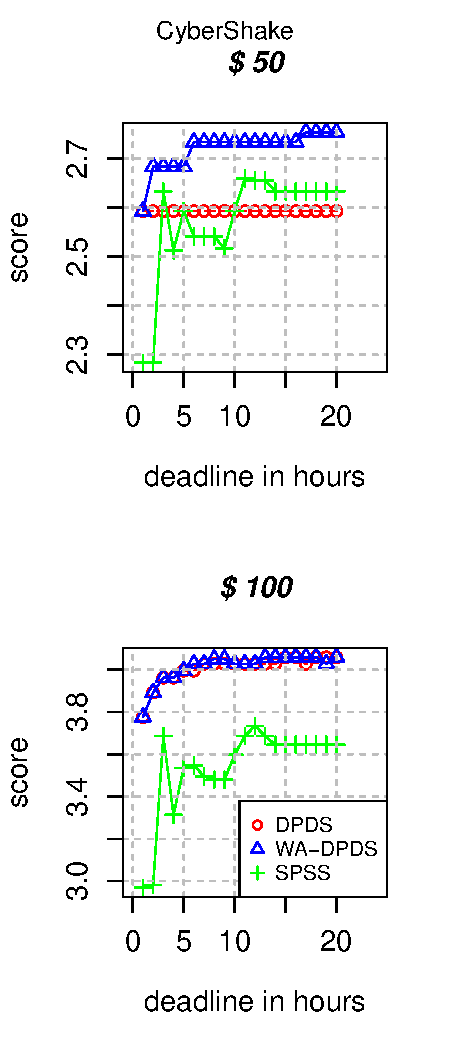
\includegraphics[width=1.0\textwidth]{figures/score-CYBERSHAKE-n-1000-8-dagh1-20m0.pdf}
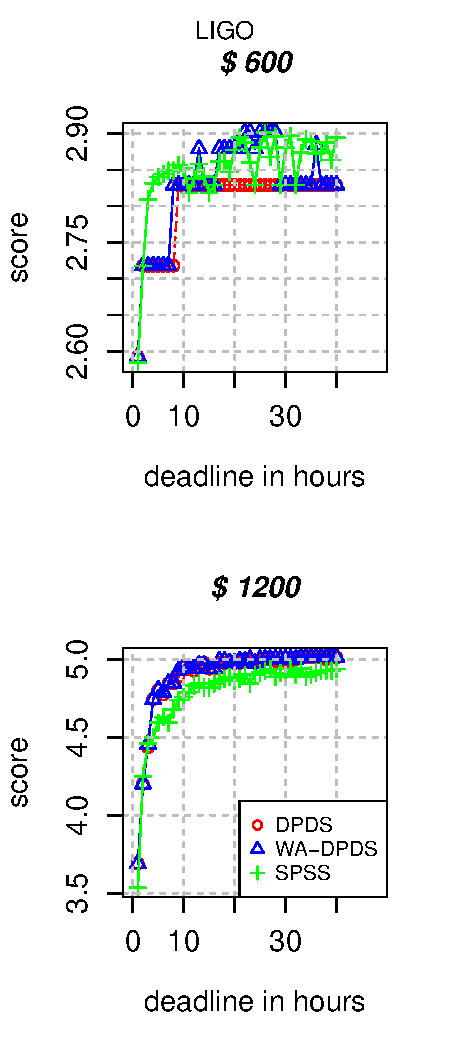
\includegraphics[width=1.0\textwidth]{figures/score-LIGO-n-1000-8-dagh1-40m0.pdf}
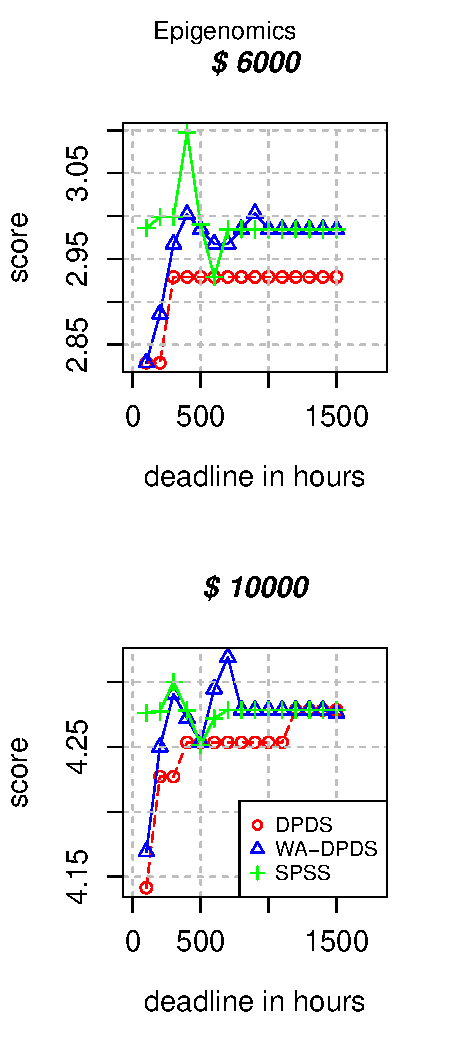
\includegraphics[width=1.0\textwidth]{figures/score-GENOME-n-1000-8-dagh100-1500m0.pdf}
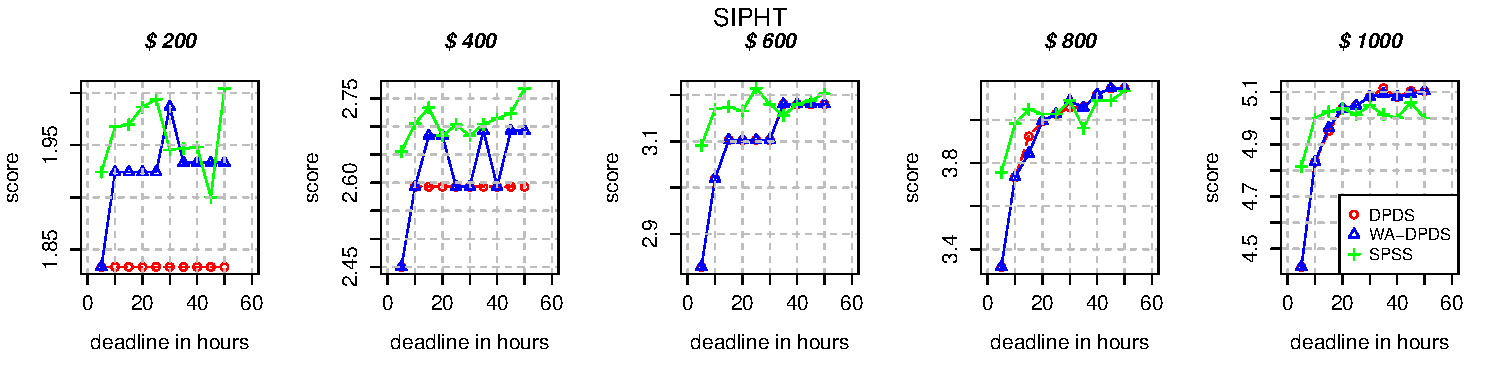
\includegraphics[width=1.0\textwidth]{figures/score-SIPHT-n-1000-8-dagh5-50m0.pdf}
\caption{Comparison of DPDS, AW-DPDS and SPSS algorithms for ensembles of 100
Pareto-distributed workflows. Score is computed as $\sum(1/(p+1))$ where
priorities of subsequent workflows are $p=0,1,2,\ldots$ (0 means highest
priority).}
\label{fig:}
\end{figure*}

\begin{figure*}[htb] 
\centering
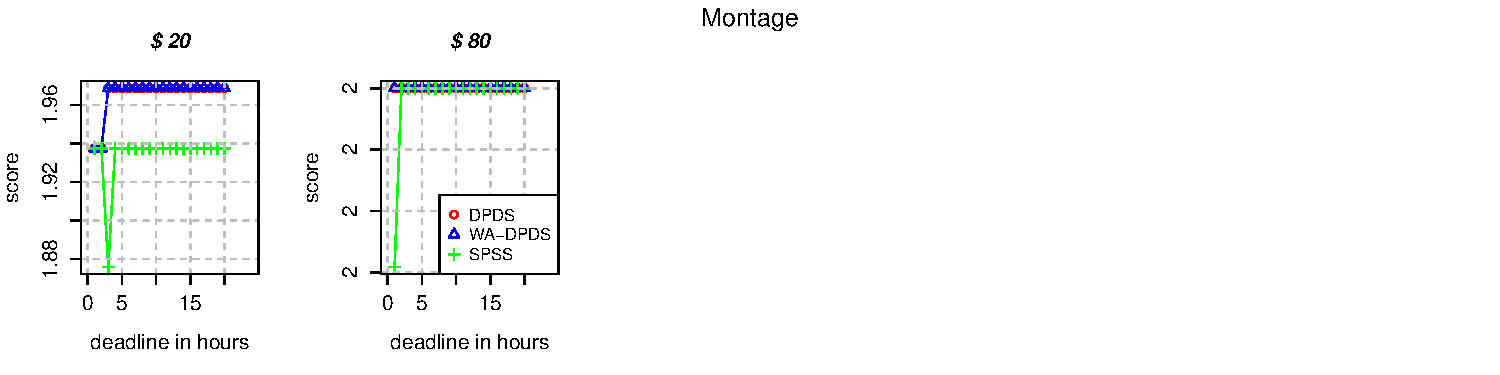
\includegraphics[width=1.0\textwidth]{figures/score2-MONTAGE-n-1000-8-dagh1-20m0.pdf}
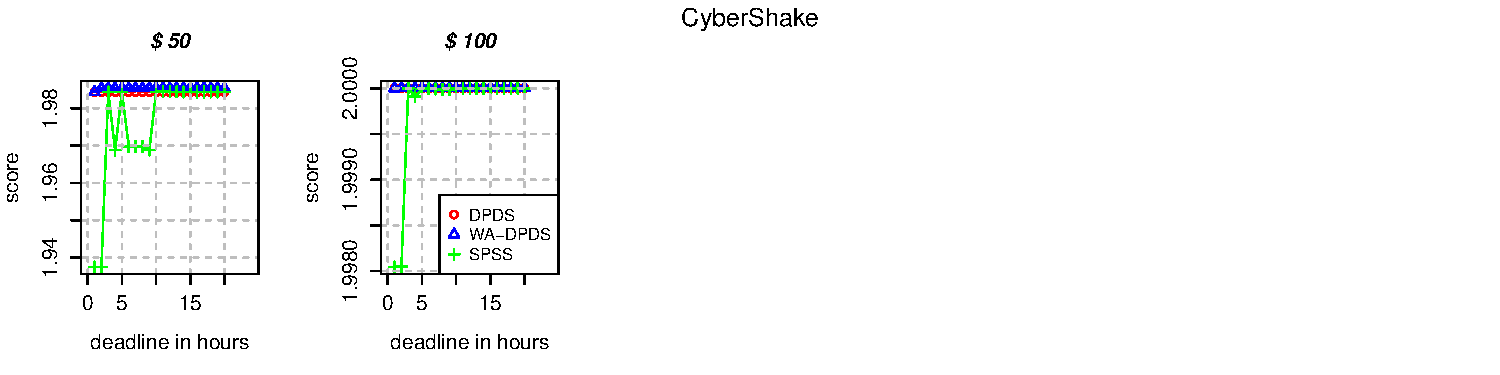
\includegraphics[width=1.0\textwidth]{figures/score2-CYBERSHAKE-n-1000-8-dagh1-20m0.pdf}
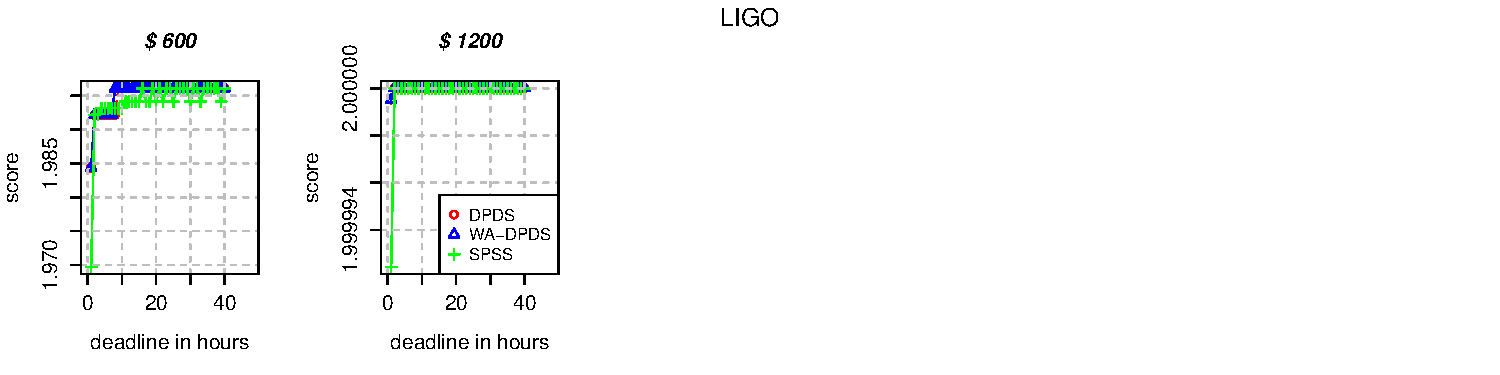
\includegraphics[width=1.0\textwidth]{figures/score2-LIGO-n-1000-8-dagh1-40m0.pdf}
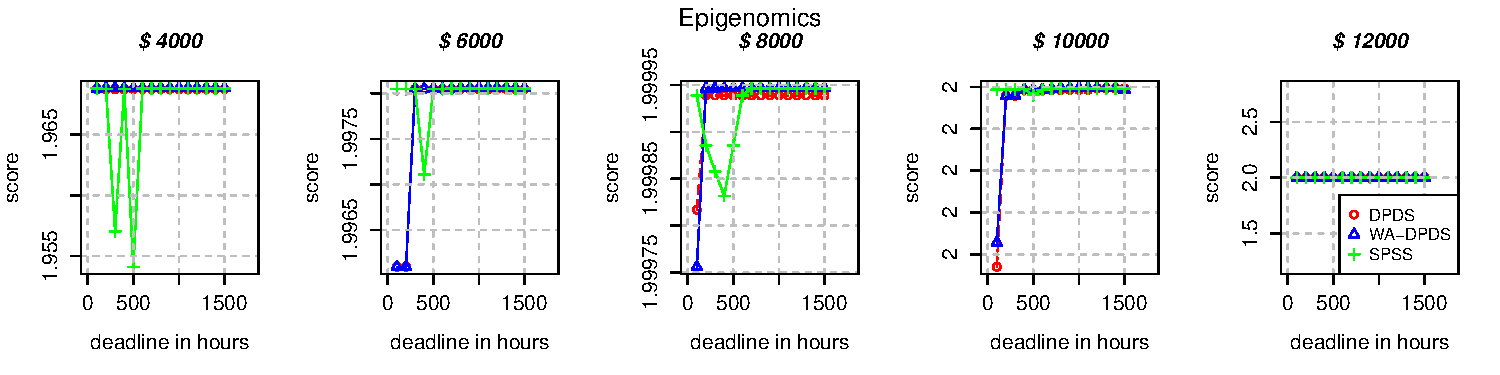
\includegraphics[width=1.0\textwidth]{figures/score2-GENOME-n-1000-8-dagh100-1500m0.pdf}
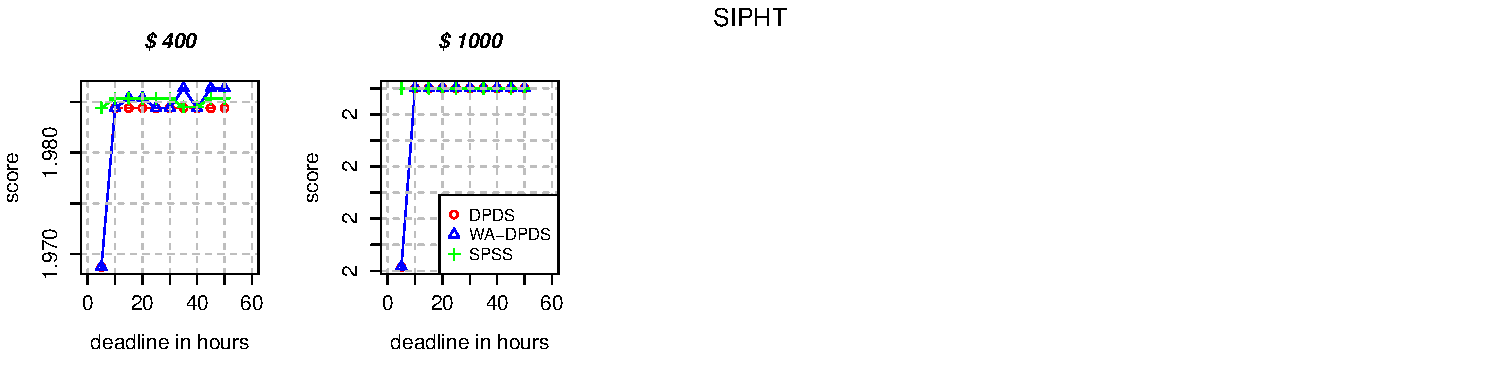
\includegraphics[width=1.0\textwidth]{figures/score2-SIPHT-n-1000-8-dagh5-50m0.pdf}
\caption{Comparison of DPDS, AW-DPDS and SPSS algorithms for ensembles of 100
Pareto-distributed workflows. Score is computed as $\sum(2^(-p))$ where
priorities of subsequent workflows are $p=0,1,2,\ldots$ (0 means highest
priority).}
\label{fig:}
\end{figure*}

\begin{figure*}[htb] 
\centering
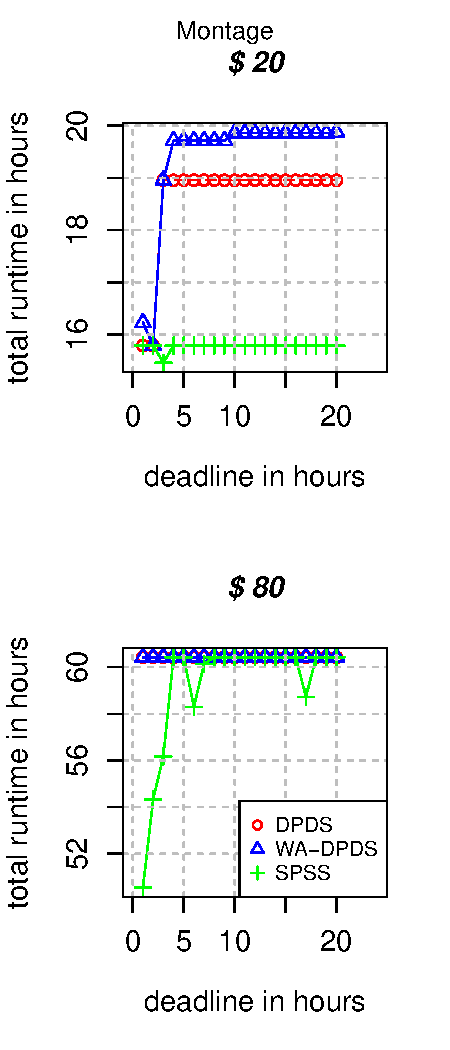
\includegraphics[width=1.0\textwidth]{figures/size-MONTAGE-n-1000-8-dagh1-20m0.pdf}
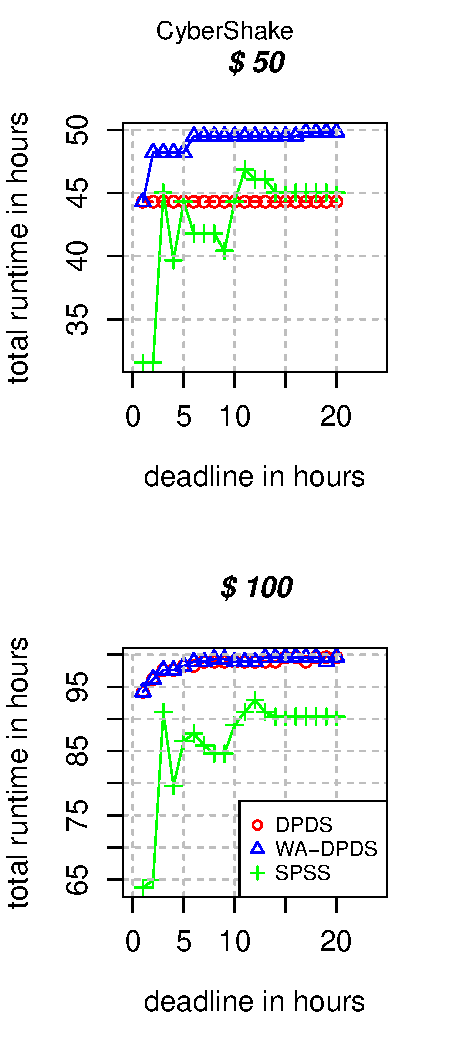
\includegraphics[width=1.0\textwidth]{figures/size-CYBERSHAKE-n-1000-8-dagh1-20m0.pdf}
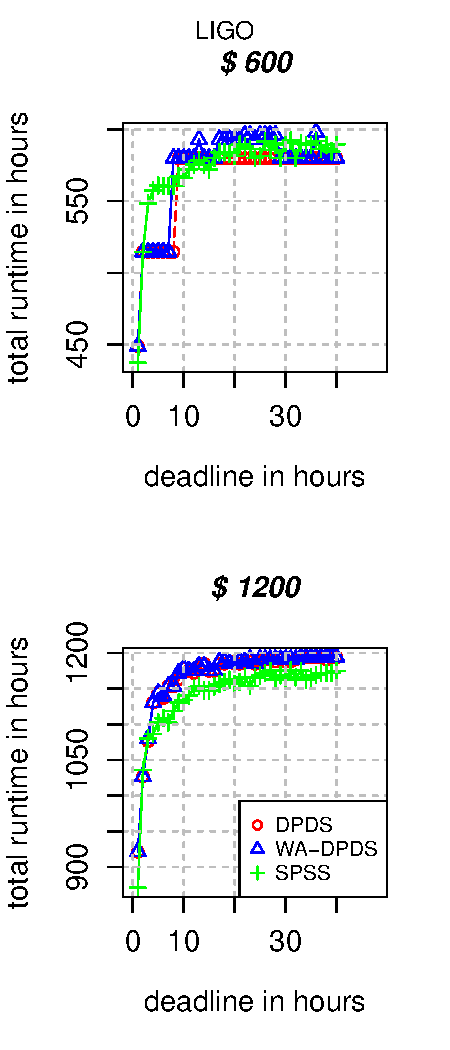
\includegraphics[width=1.0\textwidth]{figures/size-LIGO-n-1000-8-dagh1-40m0.pdf}
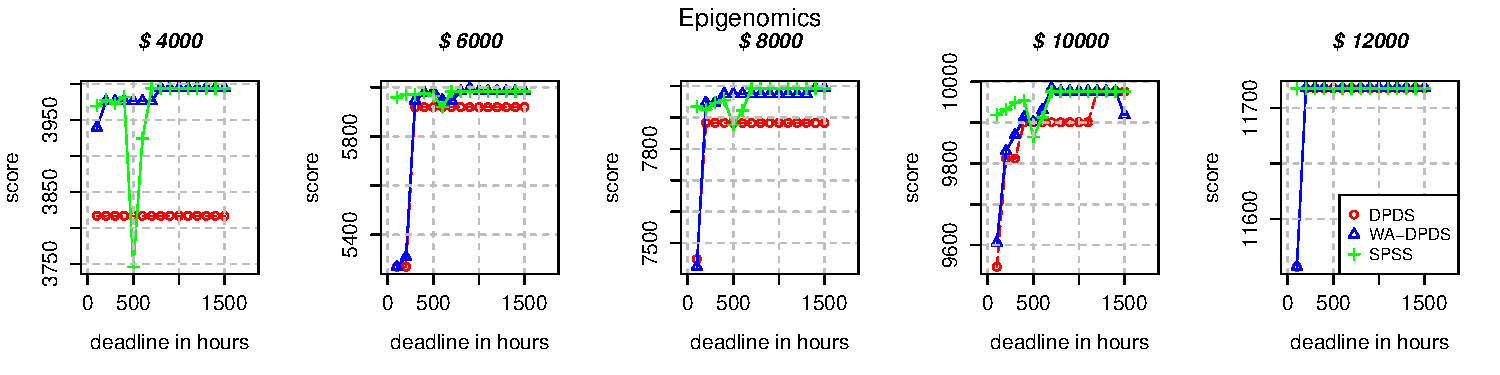
\includegraphics[width=1.0\textwidth]{figures/size-GENOME-n-1000-8-dagh100-1500m0.pdf}
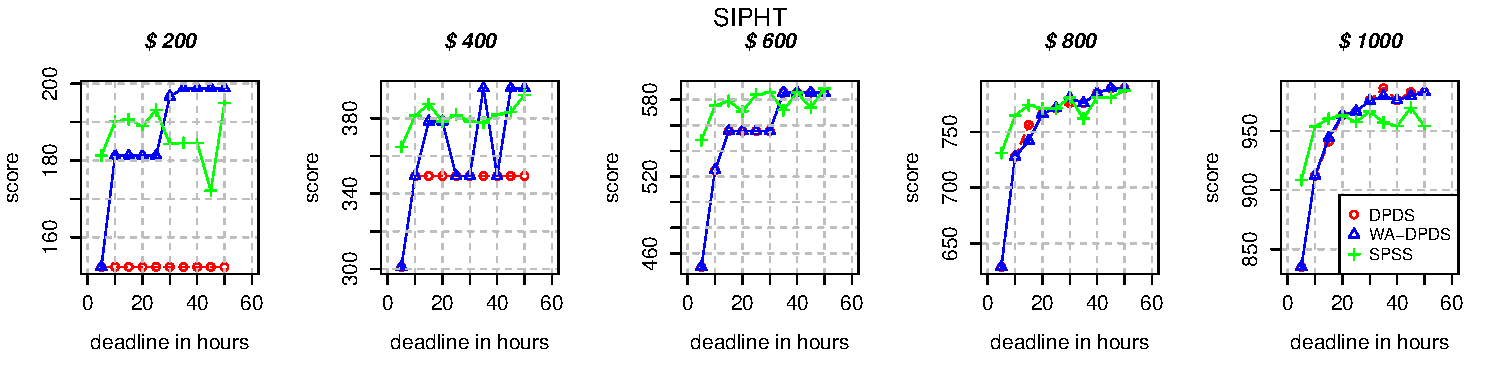
\includegraphics[width=1.0\textwidth]{figures/size-SIPHT-n-1000-8-dagh5-50m0.pdf}
\caption{Comparison of DPDS, AW-DPDS and SPSS algorithms for ensembles of 100
Pareto-distributed workflows. Score is equal to the total work completed,
i.e. it is sum of runtimes (in hours) of tasks of completed workflows.}
\label{fig:}
\end{figure*}

\begin{figure*}[htb] 
\centering
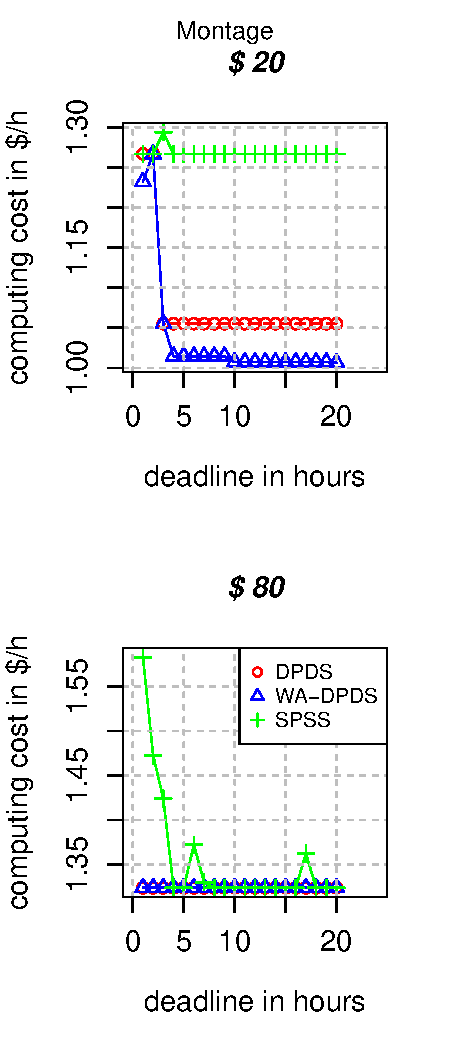
\includegraphics[width=1.0\textwidth]{figures/cost-MONTAGE-n-1000-8-dagh1-20m0.pdf}
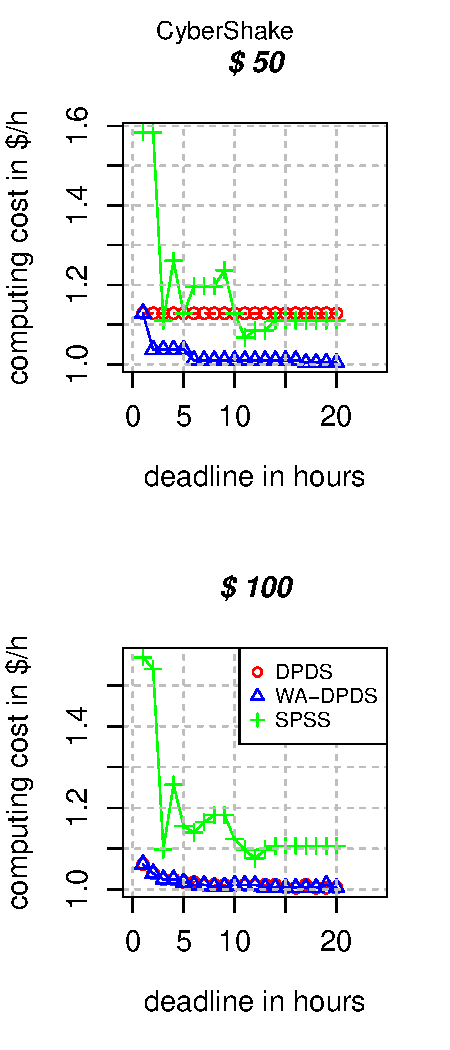
\includegraphics[width=1.0\textwidth]{figures/cost-CYBERSHAKE-n-1000-8-dagh1-20m0.pdf}
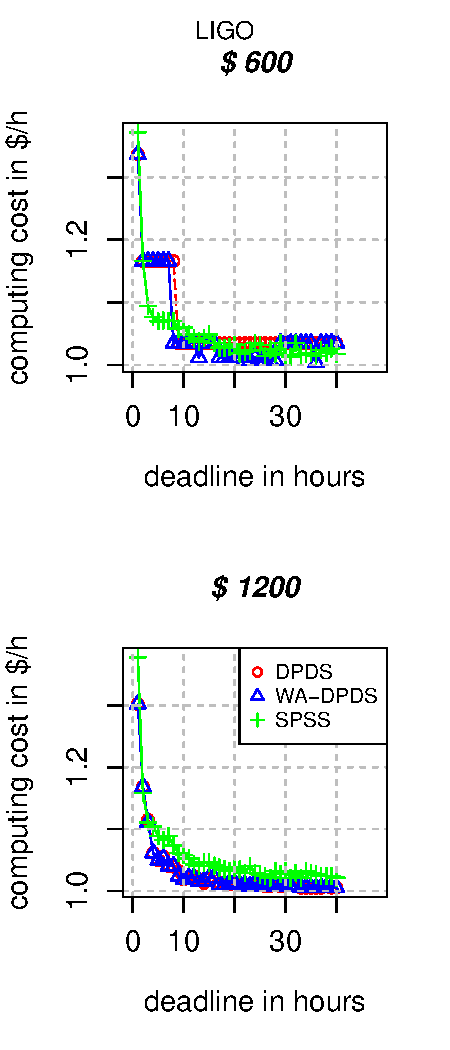
\includegraphics[width=1.0\textwidth]{figures/cost-LIGO-n-1000-8-dagh1-40m0.pdf}
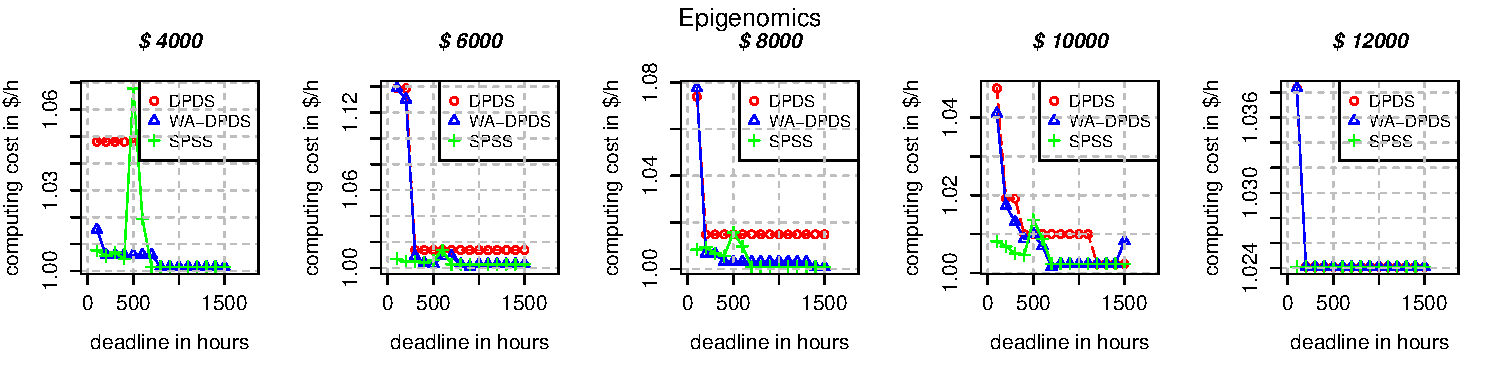
\includegraphics[width=1.0\textwidth]{figures/cost-GENOME-n-1000-8-dagh100-1500m0.pdf}
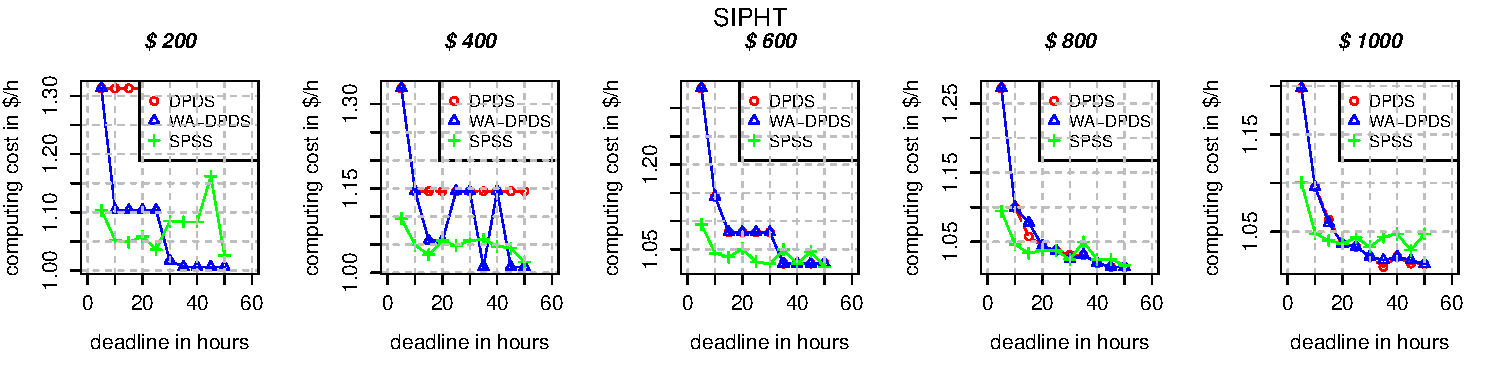
\includegraphics[width=1.0\textwidth]{figures/cost-SIPHT-n-1000-8-dagh5-50m0.pdf}
\caption{Comparison of DPDS, AW-DPDS and SPSS algorithms for ensembles of 100
Pareto-distributed workflows. Plot shows effective computing cost in \$ per
hour calclated by dividing sum of task runtimes by the total budget. Higher
cost results from lower resource utilization.}
\label{fig:}
\end{figure*}



\section{Conclusion and Future Work}


%\section{Acknowledgments}
%Acknowledgements go here.

\bibliographystyle{abbrv}
\bibliography{paper}

%\appendix
%\section{Headings in Appendices}

%\balancecolumns

\end{document}
